\documentclass[12pt]{article}
\usepackage{hyperref}
\usepackage{graphicx}
\usepackage{mathtools}
\usepackage[margin=1in, paperwidth=8.5in, paperheight=11in]{geometry}
\begin{document}
\title{Istanbul Technical University- Spring 2017 \\ BLG527E Machine Learning \\ Homework 1}
\author{Omid Abdollahi Aghdam \\
student number: 504151520\\
\href{mailto:abdollahi15@itu.edu.tr}{abdollahi15@itu.edu.tr}\\
\href{mailto:abdollahi.omid@gmail.com}{abdollahi.omid@gmail.com}
}
\date{\today}
\maketitle
\newpage
\textbf{Q1)} The code for Q1a and Q1b is written in file \textit{'q1.py'} and running the code will plot the histogram of means for all four cases, as you can see in figure 1, and will save an image file with the name '\textit{hists.png}'.\\

\begin{figure}[h]
  \centerline{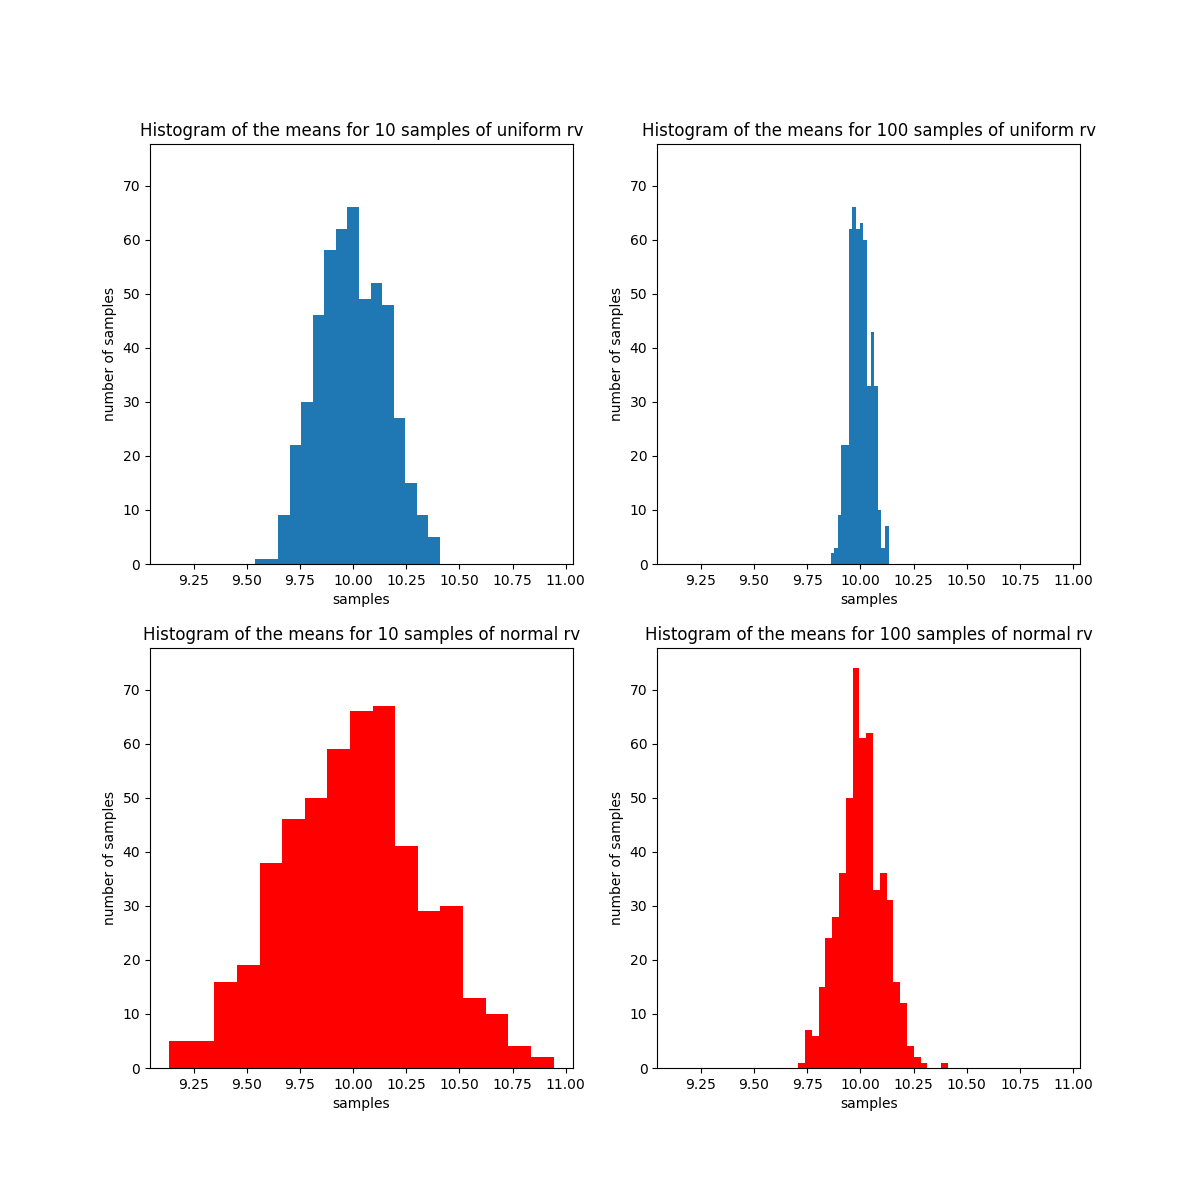
\includegraphics[width=6in]{hists.png}}
  \caption{Histograms of means.}
  \label{fig:Histograms of means}
\end{figure}
\textbf{Q1c)} According to Central Limit Theorem, if we take $N$ sample from any distribution with mean $\mu$ and variance $\sigma^2$, calculate the mean of samples, and repeat this experiments several times, in this homework we repeat 500 times. As a result, the distribution of the mean  get closer to a Normal Distribution with mean $\mu$ and variance $\sigma^2/N$ as the number of samples $N$ increases.\\
\newpage
\textbf{Similarities:}
\begin{enumerate}
\item All four plots looks like normal distribution, and as the number of samples increases to 100 the histograms become more similar to Normal distribution pdf.
\item The mean of all histograms are $\mu=10$ because the mean of distributions which we draw random samples from equal 10.
\item The variance of sampling distribution of means get closer to each other as $N$ increases, so, the variance of histograms for $N=100$ are closer to each other than histograms for $N=10$.
\end{enumerate}
\textbf{Differences:}
\begin{enumerate}
\item The only difference I can see is the variances. However as the $N$ increases the differences become less significant.
\end{enumerate}


\textbf{Q2) a)} We have the discriminant function as follow:
\begin{equation} \label{disc_func}
g_{i}=\ln(p(x|w_{i})) + \ln(p(w_{i}))\\
\end{equation}
Also we have:
\begin{gather*}
x \in \Re \\ 
class1: x\sim\mathbf{N}(\mu_{1},\sigma)\\
class2: x\sim\mathbf{N}(\mu_{2},\sigma)\\
p(w_{1})=p(w_{2})
\end{gather*}

Using the information above and the following equation we can derive discriminant functions for class 1 and class 2.
\begin{equation}
p(x|w_{i})=\frac{1}{\sqrt{2\pi}\sigma_{i}}exp\left[-\frac{(x-\mu_{i})^2}{2\sigma_{i}^2} \right]
\end{equation}
Now we plug in the equation 2 in equation 1 and derive discriminant functions.

\begin{equation}
g_{1}(x)=\ln\left[\frac{1}{\sqrt{2\pi}\sigma}exp\left[-\frac{(x-\mu_{1})^2}{2\sigma^2} \right]\right] + \ln(p(w_{1}))
\end{equation}
We use logarithm properties to derive the discriminant function for class 1, $g_{1}(x)$, and later we just replace $\mu_{1}$ with $\mu_{2}$ to get the discriminant function for class 2, $g_{2}(x)$.
\begin{gather*}
	g_{1}(x)=\ln(1) -\frac{1}{2}ln(2\pi)-ln(\sigma)-\frac{(x-\mu_{1})^2}{2\sigma^2}ln(e)+ln(p(w_{1}))\\
	g_{1}(x)=-\frac{1}{2}ln(2\pi)-ln(\sigma)-\frac{(x-\mu_{1})^2}{2\sigma^2}+ln(p(w_{1}))
\end{gather*}

The discriminant functions for class 1 and class 2 are:

\begin{equation}
	g_{1}(x)=-\frac{1}{2}ln(2\pi)-ln(\sigma_{1})-\frac{(x-\mu_{1})^2}{2\sigma_{1}^2}+ln(p(w_{1}))
\end{equation}
\begin{equation}
	g_{2}(x)=-\frac{1}{2}ln(2\pi)-ln(\sigma_{2})-\frac{(x-\mu_{2})^2}{2\sigma{2}^2}+ln(p(w_{2}))
\end{equation}

\textbf{b)} To find the separation surface we set discriminant equations equal.
\begin{equation}
g_{1}(x)=g_{2}(x)
\end{equation} 
Now we replace equation 4 and equation 5 in equation 6 and find the equation for separating surface.

\begin{gather*}
	-\frac{1}{2}ln(2\pi)-ln(\sigma_{1})-\frac{(x-\mu_{1})^2}{2\sigma_{1}^2}+ln(p(w_{1}))=-\frac{1}{2}ln(2\pi)-ln(\sigma_{2})-\frac{(x-\mu_{2})^2}{2\sigma_{2}^2}+ln(p(w_{2}))
\end{gather*}
\begin{equation}
	\left(\frac{1}{2\sigma_{2}^2}-\frac{1}{2\sigma_{1}^2}\right)x^2+\left(\frac{\mu_{1}}{\sigma_{1}^2}-\frac{\mu_{2}}{\sigma_{2}^2}\right)x+\frac{\mu_{2}^2}{2\sigma_{2}^2}-\frac{\mu_{1}^2}{2\sigma_{1}^2}+\ln\frac{\sigma_{2}}{\sigma_{1}}+\ln\frac{p(w_{1})}{p(w_{2})}=0
\end{equation}
As you can see separating surface function is a quadratic function ($ax^2+bx+c=0$) and we can find its roots using the following formula.
\begin{center}
$x1,x2=\frac{-b\pm\sqrt{b^2-4ac}}{2a}$
\end{center}
In this example $\sigma_{1}=\sigma_{2}$, so $a=0$ so we can eliminate quadratic term. The new separating surface equation can be written as follow:
\begin{equation}
	x=\frac{2\sigma^2\ln\left(\frac{p(w_{2})}{p(w_{1})}\right)+\mu_{1}^2-\mu_{2}^2}{2(\mu_{1}-\mu_{2})}
\end{equation}
\newpage
\textbf{c)} We plug $\mu_{1}=5$, $\mu_{2}=15$, $\sigma=5$ and $p(w_{1})=p(w_{2})=0.5$ in equation 8. As a result we have the following vertical line as the separating surface. You can see the plot in figure 2. Separating line specifies which class the inputs belong to. The code is written in \textit{'pdfs.py'}.
\begin{center}
	$x=10$
\end{center}
\begin{figure}[h]
  \centerline{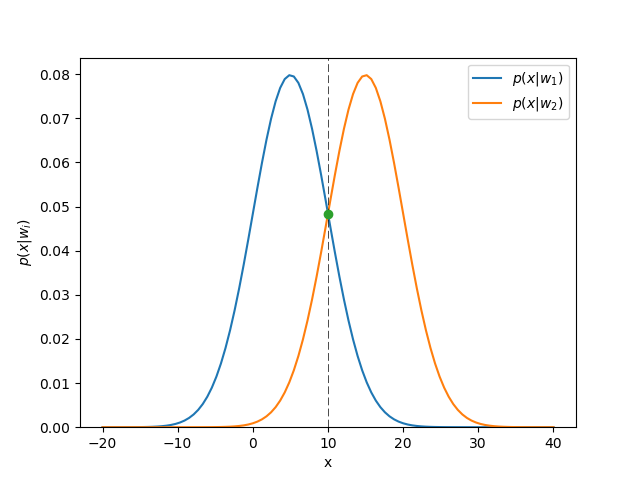
\includegraphics[width=3.5in]{pdfs.png}}
  \caption{pdf's of the two classes and separating surface, $x=10$.}
  \label{fig:Pdf's of classes pw1=pw2}
\end{figure}
\newpage
\textbf{d)} We plug the new class probabilities $p(w_{1})=0.8$ and $p(w_{2})=0.2$ in the equation 8 and the new separating surface is \textbf{x=13.4657}.The new plot is shown in figure 3.
\begin{figure}[h]
  \centerline{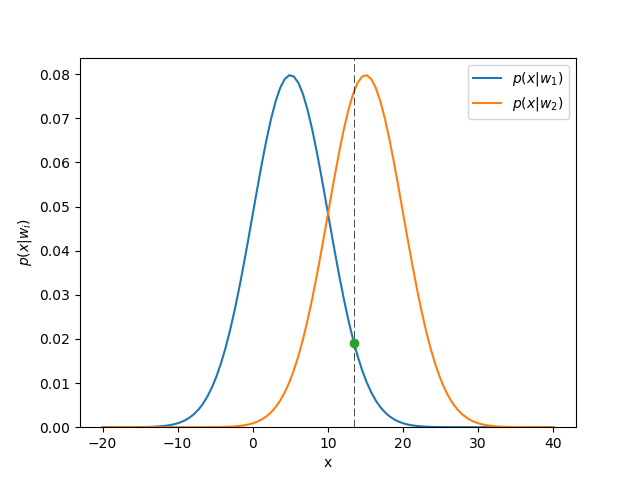
\includegraphics[width=3.5in]{pdfs1.png}}
  \caption{pdf's of the two classes and separating surface, $x=13.4657$.}
  \label{fig:Pdf's of classes pw1=0.8}
\end{figure}\\*
\textbf{e)} As $p(w_{2})=p(w_{1})$ in \textbf{c)} so we generate equal number of samples for datasets. We generated 200 samples from each distribution. Finally, we use the mean and standard deviation of generated datasets and plug them in equation 7 to calculate the separating point. The equation has two results we select the result that is in range of the generated x values. The histograms are shown in figure 4.
 \begin{figure}[h]
  \centerline{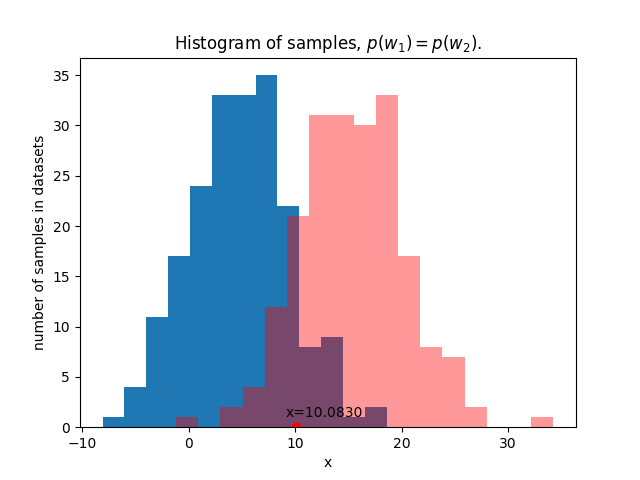
\includegraphics[width=3.5in]{hist05.png}}
  \caption{The histograms of generated datasets .}
  \label{fig:Histograms pw1=pw2}
\end{figure}\newpage
For \textbf{d)} we generated 320 samples from class 1 and 80 samples from class 2. We calculate the separating point using equation 7 and select the x that is in the range of generated x values. The histograms for the generated datasets are shown in figure 5. 
 \begin{figure}[h]
  \centerline{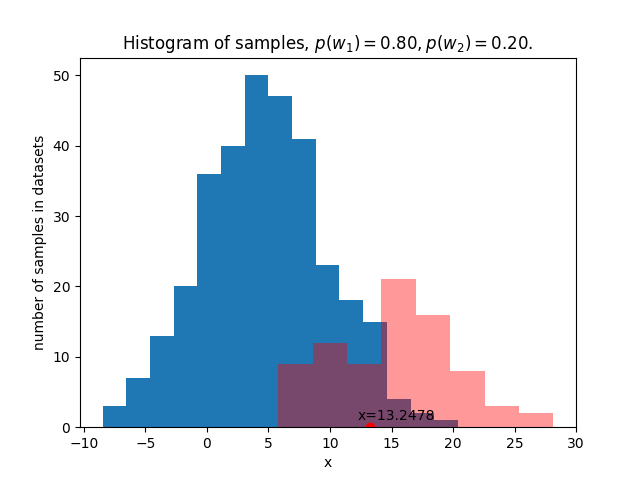
\includegraphics[width=3.5in]{hist08.png}}
  \caption{The histograms of generated datasets .}
  \label{fig:Histograms pw1=pw2}
\end{figure}\\
Source codes for the first question is written in file \textit{'q1.py'} and the codes for the second question is written in file \textit{'q2.py'}. In order to run codes successfully \textit{numpy, matplotlib, scipy} python libraries must have been installed in your system. 
\end{document}